% !TEX root = ../Thesis.tex

\chapter{Introduction}\
\label{ch:introduction}



\section{Motivation and Literature Review}\
\label{ch:motivation}
%(Context and justification, why is this work important?)\\

In December 2015, the COP21 agreement was signed by 195 countries, setting a legally binding goal of reducing greenhouse gases such as not exceed 1.5\textsuperscript{o}C. The agreement covers accountability, transparency and better reporting of emissions, greater effort towards adaptation and improving the resilience of cities, reducing emissions, and supporting sustainable practices in developing countries. Many developed countries have been tackling energy efficiency in buildings since the 1980s. The inclusion developing countries, particularly those with the fastest growth rates, in COP21 agreements adds huge reduction potential for global energy and GHG reductions within the building industry.
 
Improving energy efficiency in buildings does more than just reduce greenhouse gas emissions. It also comes with cost savings and increased earnings for energy exporting countries, improved energy security and higher productivity for businesses\cite{EIA}. In 2014, the global energy efficiency market was worth approximately \$90 billion. The projected increase to \$125 billion by 2020, which is expected to be driven mainly by energy policy, would still fall short of the \$215 billion required to reach just the 2\textsuperscript{o}C target\cite{EIA}. Policy alone will not be enough to achieve the 2\textsuperscript{o}C target; it is necessary that current research and development focuses on increasing the ease and attractiveness of measures that reduce building energy demand.\par 

Building energy models are essential tools for predicting the performance of new construction and refurbishments, measured in terms of additional energy required to maintain comfortable internal temperatures, which are a function of outdoor temperature, building properties and interior energy gains. Building performance predictions are necessary in the evaluation of intervention possibilities return on investment. Models are also sometimes used in energy certification of existing buildings, with other approaches being computational (using input collected data by an energy auditor) and performance-based (using bills).\par

Deterministic models are based on heat transfer theory, making use of physical characteristics and well-established models of subprocesses to simulate buildings in discrete time. The problem with these models is that predicted temperatures and loads are fixed for given inputs, making it impossible to correct the prediction using measured data. This makes it difficult to predict the accuracy of such models, since information about physical parameters is partly hidden in the parametrization \cite{madsen1995estimation}.\par

One possible solution to the problem of model accuracy is the use of stochastic models, also referred to as \textit{grey box models}. These models combine statistics with knowledge of physical properties, described by a set of first-order stochastic differential equations, commonly referred to as a stochastic linear state-space model in continuous time \cite{bacher2011identifying}. The physical properties of these \textit{Resistor-Capacitor} (RC) models are modeled as a thermal equivalent to an electrical circuit, with temperature as voltage, heat flux as current, conductance as thermal conductance, and thermal mass as capacitance \cite{sonderegger2010diagnostic}. By using lumped parameters, this configuration requires less information about physical properties than deterministic methods, where detailed parametrization of elements is required. Instead, an additive noise term term is added to the parametrization to correct for modeling approximations, unrecognized and unmodeled inputs, and noise-corrupted measurements of the inputs using measured data \cite{madsen1995estimation}.\par

It is important to highlight the distinction between simulation and forecasting, where simulation assumes undisturbed outputs and forecasting includes a recursive calibration with measured outputs \cite{mejri2011energy}. Forecasting applications include integration of renewable energies, implementation of electrical heating coupled with thermal storage, the inclusion of wind effects on airtightness \cite{bacher2011identifying}, and assessment of variation between houses to assess building flaws \cite{sonderegger2010diagnostic}.\par 

The literature cited above offers detailed explanations of the statistical approaches to model verification for forecasting. This topic, however, falls out of the scope of the report, since the RC model developed in this project is only used for simulation. The next sections contain an overview and comparison of three model definitions, and an introduction to the use case.

\newpage
\section{Resistor-Capacitor Models}\
\label{ch:RC Models}

This section deals with the use of RC models for single zones. RC models are not readily adaptable for multi-zone calculation because the formulation of zone coupling adds another layer of complexity. This would somewhat offset  the benefits of using RC models as opposed to conventional deterministic models, which are sufficiently developed to handle multiple zones.\par

In single-zone configuration, RC models are assumed to be connected adiabatically to neighboring zones. The thermal system is modeled based on the energy balance equation, which in its simplest form states that: 

\begin{equation} \label{eq:1}
\textrm{Heat in} = \textrm{Heat out} + \textrm{Heat stored}
\end{equation}

This holds true for any given location or node in the system, such that the heat into the node is equal to the heat out of the node plus any heat that is stored \cite{SysThermalModel}. To illustrate this, one may consider a closed box with capacitance $C_m$ and resistance $R_1$, represented in the circuit diagram in \ref{fig:1R1C_Model} below:

\begin{figure}[ht]
      \begin{center}
          \begin{circuitikz}
            \draw (0,0)
            node[label={left:$T_e$}] {}
            to[short,*-] (1,0)
            to[short] (1,1)
            to[R=$R_1$] (3,1) % The voltage source
            node[label={right:$T_m$}] {}
            to[C=$C_m$,*-] (3,-1)
            to[short] (1,-1)
            to[short] (1,0);
          \end{circuitikz}
          \caption{A 1R1C Model of a single zone}
      \label{fig:1R1C_Model}
      \end{center}
\end{figure}



Using this principle, the electrical circuit laws may be translated to their thermal equivalent as follows: 


\begin{equation} \label{eq:2}
Q = \frac{T_m-T_e}{R_1}
\end{equation}

\begin{equation} \label{eq:3}
C_m \frac{dT_m}{dt} = Q
\end{equation}

Where $T_R$ is the temperature difference across the resistor and $T_C$ is the temperature difference across the capacitor. Because there is no heat input, \ref{eq:1} reduces to:

\begin{equation} \label{eq:4}
0 = \frac{T_m-T_e}{R_1} + C_m \frac{dT_m}{dt}
\end{equation}

Which can be simplified to:

\begin{equation} \label{eq:5}
\frac{dT_m}{dt} = \frac{T_e-T_m}{R_1 C_m}
\end{equation}

This leads to a \textit{separable} differential equation, which may be solved numerically using finite difference methods such as the \textit{Crank-Nicholson} method in a stable manner. The \textit{Crank-Nicholson}(\ref{eq:8}) is a combination of the less accurate \textit{forward Euler}(\ref{eq:6}) and \textit{backward Euler}(\ref{eq:7}) methods.

\textit{forward Euler}:
\begin{equation*}
{dT_m} = \frac{T_e-T_m}{R_1 C_m} {dt}
\end{equation*}

\begin{equation}\label{eq:6}
\rightarrow T_{m+1} = \left[\frac{T_e-T_m}{R_1 C_m}\right] \Delta{t} + T_m
\end{equation}

\textit{backward Euler}:
\begin{equation*}
T_{m+1} = \left[\frac{T_e-T_{m+1}}{R_1 C_m}\right] \Delta{t} + T_m
\end{equation*}

$Let$ \alpha = \frac{R_1 C_m}{\Delta{t}} : 

\begin{equation*}
\alpha T_{m+1} = T_e-T_{m+1} + \alpha T_m 
\end{equation*}

\begin{equation*}
(\alpha+1) T_{m+1} = T_e + \alpha T_m 
\end{equation*}

\begin{equation*}
T_{m+1} = \frac{T_e + \alpha T_m}{\alpha+1} 
\end{equation*}

\begin{equation} \label{eq:7}
\rightarrow T_{m+1} = \frac{T_e \delta{t} + R_1 C_m Tm}{R_1 C_m + \Delta{t}} 
\end{equation}


\textit{Crank-Nicholson}:

\begin{equation*}
T_{m+1} - T_m = \frac{1}{2} \left[ \left[ \frac{T_e-T_m}{R_1 C_m}\right] + \left[ \frac{T_e-T_{m+1}} {R_1 C_m}\right] \right] \Delta{t}
\end{equation*}

$Let$ \alpha = \frac{R_1 C_m}{\Delta{t}} : 


\begin{equation*}
2 \alpha T_{m+1} - 2 \alpha T_m = T_e - T_m + T_e - T_{m+1}
\end{equation*}

\begin{equation*}
(2 \alpha + 1) T_{m+1} = 2 T_e + T_m (2 \alpha - 1) 
\end{equation*}

\begin{equation*}
T_{m+1} = \frac{2 T_e + T_m (2 \alpha - 1)}{(2 \alpha + 1)} 
\end{equation*}


\begin{equation} \label{eq:8}
T_{m+1} = \frac{2 T_e \Delta{t} + T_m (2 R_1 C_m + \Delta{t})}{(2 R_1 C_m + \Delta{t})} 
\end{equation}

Thus the internal temperature can be computed for a given external operative temperature at any time step. The graphs below illustrate the use of forward-Euler, backward-Euler and Crank-Nicholson methods to solve the differential equation.\par



\begin{figure}[ht] %h can be omitted for better page layout
  \begin{center}
    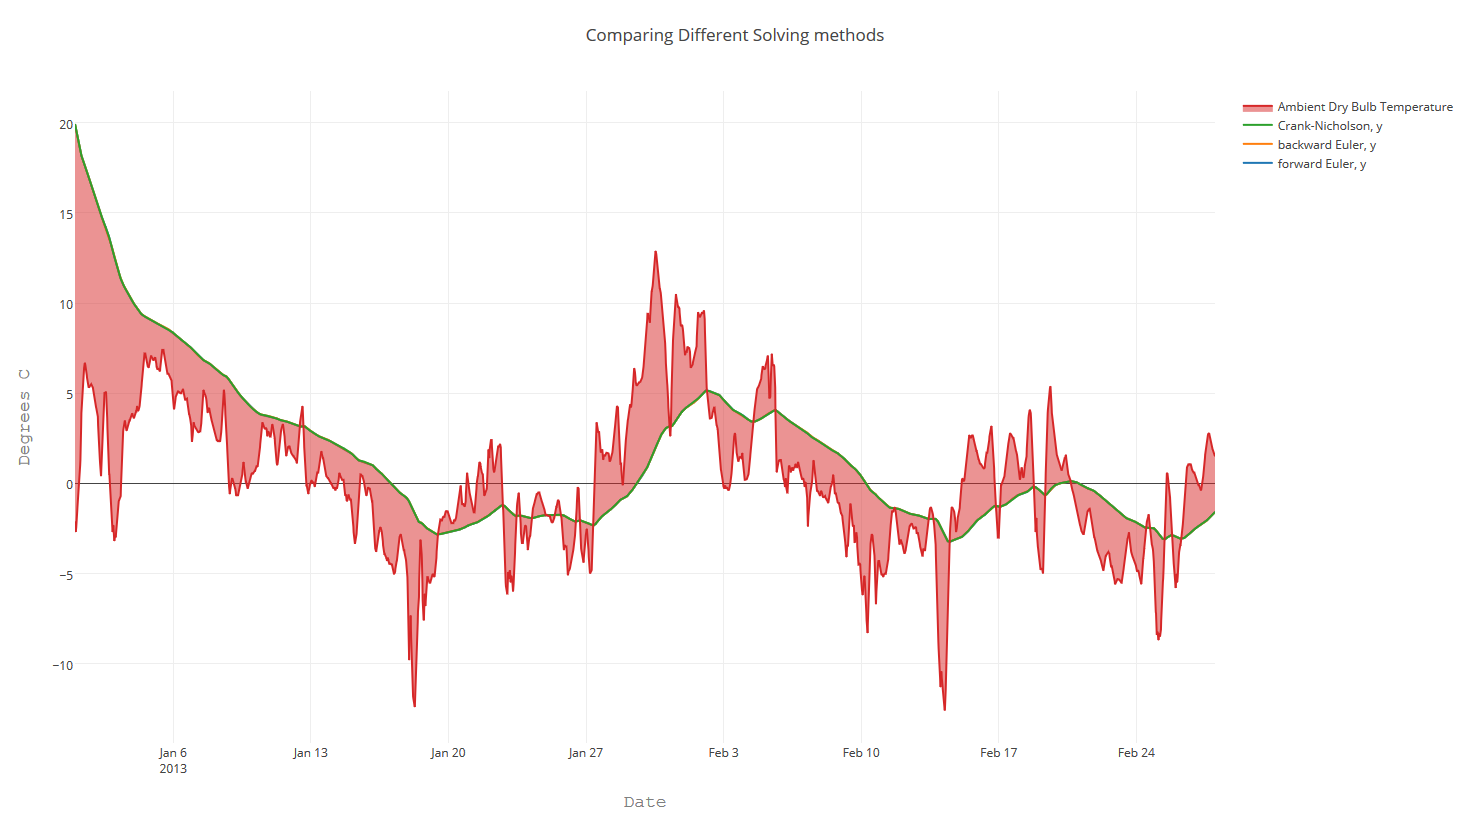
\includegraphics[width=\textwidth, trim= 0cm 0cm 0cm 0cm,clip]{temperatures.png}
    \caption{T_{ext} $ and $ T_{int} $ for a 1R1C model$}
    \label{fig: 1R1C model}
  \end{center} 
\end{figure}




\newpage
The Crank-Nicholson approach takes the average result of FE and BE methods. \ref{fig: FE and BE error} shows the relative error of the two methods.

\begin{figure}[ht] %h can be omitted for better page layout
  \begin{center}
    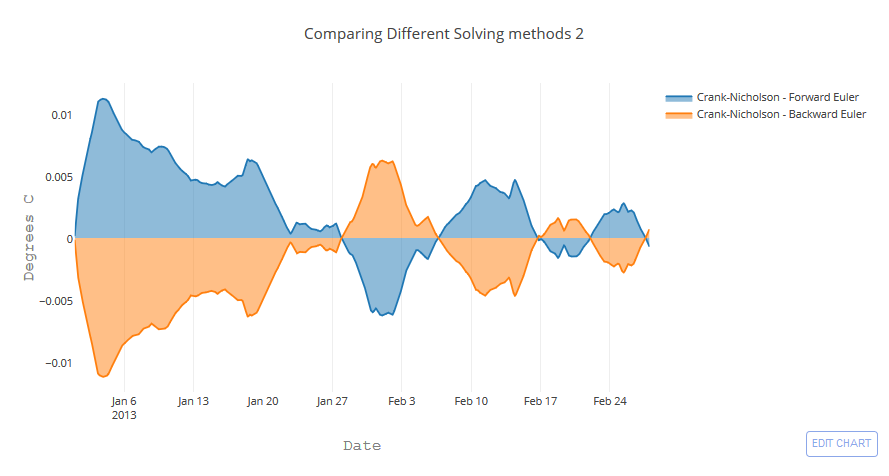
\includegraphics[width=\textwidth, trim= 0cm 0cm 0cm 0cm,clip]{error.png}
    \caption{Error for FE and BE relative to CN}
    \label{fig: FE and BE error}
  \end{center} 
\end{figure}

\newpage

The model can be extended to account for heat loss due to ventilation and infiltration, as well as solar gains, internal gains and system heating and cooling, using a PI controller. The heat losses are modeled as additional resistances while the internal gains are energy added to the system.\par

\begin{figure}[ht]
      \begin{center}
          \begin{circuitikz}
            \draw (0,1)
            node[label={left:$T_e$}] {}
            to[short,*-] (1,1)
            to[short] (1,2)
            to[short] (2,2) 
            to[R=$R_{infl}$,*-] (4,2) % The voltage source
            to[short,*-] (5,2)
            node[label={$T_m$}] {}
            to[C=$C_m$,*-] (5,0)
            to[short,*-] (5,-1)
            to[short] (1,-1)
            to[short] (1,1);

            \draw[short](2,2)
            to[short] (2,3)
            to[R=$R_{vent}$] (4,3)
            to[short] (4,2);

            \draw[short](2,2)
            to[short] (2,1)
            to[R=$R_{env}$] (4,1)
            to[short] (4,2)
            to[short] (5,2);

            \draw[short](5,2)
            to[short,](7,2)
            to[european current source,l=$\phi_{Heat}$](7,0)
            to[short](5,0);
            
            \draw[short](7,2)
            to[short,](9,2)
            to[european current source,l=$\phi_{Rad}$](9,0)
            to[short](7,0);
            
            \draw[short](9,2)
            to[short](11,2)
            to[european current source,l=$\phi_{Int}$](11,0)
            to[short](9,0);

            %\draw[short](5,2)
            %to[european current source,l_=$\phi_{HC}$] (3,5);

          \end{circuitikz}
          \caption{A 3R1C Model of a single zone}
      \label{fig:1R1C_Model}
      \end{center}
\end{figure}

Equation \ref{eq:9} shows the Forward-Euler differential equation for a 3R1C Model.

\begin{equation} \label{eq:9}
T_{m+1} =  T_m + \left(\frac{Q_{int} + Q_{heat} + Q_{cool}}{C_m} + \frac{1}{C_m R_i} [T_e - T_m] \right)\Delta{t}
\end{equation}

The 5R1C model shown in figure \ref{fig:5R1C_Model} below is specified in ISO13790, Annex B\cite{ISO13790}}. In this case, the resistances are modeled as capacitances (1/Resistance). H\textsubscript{ve} replaces R\textsubscript{vent} and R\textsubscript{inf} as the transmission coefficient due to ventilation and infiltration. Four more conductances are added: H\textsubscript{tr,\textit{is}}, the coupling conductance between the air and surface node, H\textsubscript{tr,\textit{w}} and H\textsubscript{tr,\textit{op}}, the transmission coefficients of glazed and opaque elements, respectively, and H\textsubscript{tr,\textit{em}} the combination of the previous two. Since the equations are readily accessible in the code, they have been omitted from this report.


\begin{figure}[ht]
\begin{center}
    \begin{circuitikz}
      \draw (0,0)
      node[label={left:$T_e$}] {}
      to[short,*-] (1,0)
      to[short] (1,1)
      to[european resistor=$H_w$] (3,1); % The resistor

      \draw(1,0)
      to[short] (1,-1)
      to[european resistor=$H_{em}$] (3,-1)
      node[label={10:$T_m$}] {}
      to[european resistor,l_=$H_{ms}$] (3,1)
      node[label={10:$T_s$}] {}
      to[european resistor,l_=$H_{is}$] (3,3)
      node[label={10:$T_{air}$}] {}
      to[european resistor,l_=$H_{ve}$] (1,3)
      to[short,-*] (0,3)
      node[label={left:$T_{sup}$}] {};

      \draw(3,-1)
      to[short,*-] (5,-1)
      to[short] (5,1)
      to[short,-*] (3,1);

      \draw(5,1)
      to[short] (5,3)
      to[short,-*] (3,3)
      to[european current source,l_=$\phi_{HC}$] (3,5);

      \draw(5,1)
      to[european current source,l_=$\phi_{sol}+\phi_{int}$] (7,1);

      \draw(3,-1)
      to[C=$C_m$] (3,-2)
      node[ground]{};


    \end{circuitikz}
    \caption{A 5R1C Model of the single zone office space}
\label{fig:5R1C_Model}
\end{center}
\end{figure}


The 5R1C was adopted for the simulations to avoid carrying out verification on a bespoke model, especially since no building data was available for such verification. A comparison of the parameters used by the 1R1C, 3R1C and 5R1C can be found in \ref{fig: Comparison of thermal parameters for RC models described}. THE PLOTS BELOW compare the performance of the 3R1C and 5R1C, which were implemented in Python by Prageeth Jajathissa.


\newpage
\section{Use Case: The Adaptive Solar Facade and CEA Archetypes}\

The adaptive solar facade *reference not working* (ASF) is a soft-robotic actuated array of diamond-shaped PV panels, designed to be combined with glazed facade elements. Since its inception at the \textit{Chair of Architecture and Building Systems}, ETH Zurich in 2011, it has been the subject of several publications, theses and semester projects; with topics varying from mechanical optimization, computational analysis methods and lifecycle analysis. Two prototypes have already been built; one on the House of Natural Resources at ETH Honggeberg, and a demonstration array at the chair of Architecture and Building Systems. Furthermore, two new arrays are under construction for the Nest HILO Facade *CITATION* \par

The high degrees of freedom of each panel poses a challenge to the control and modeling of the system. The configuration could be optimized for heating, cooling, lighting, total energy, or even views. To guarantee maximum amenity, the long term vision is to design an interface where occupants can choose their preferred optimization settings or even manually override 

Originally modeled in Rhinoceros using Grasshopper and Ladybug, the platform has proven to be unwieldy when it comes to repeated use: while the software is open source, the nested softwares make it hard to fully access and modify the code. Another problem is that the software is Windows-based, which rules out the use of supercomputers for expensive simulations or cheap micro-computers such as Raspberry PI for operational computations.\par

\begin{figure}[h] %h can be omitted for better page layout
  \begin{center}
    
\includegraphics[width=\textwidth, trim= 0cm 0cm 0cm 0cm,clip]{asf.png}
    \caption{An early prototype of the ASF installed on the House of Natural Resources}
    \label{fig: ASF}
  \end{center} 
\end{figure}

As a result, there is an ongoing research vein focused on converting the grasshopper scripts into a more powerful and transferable Python code. Of particular relevance to this report is the \textit{Numerical Analysis of the Adaptive solar Facade}, an ongoing thesis project by Mauro Luzzatto. Luzzatto's project is investigating optimal configurations of the ASF for lighting, heating, cooling, PV generation and total energy. While Luzzatto's research deals more with modelling the ASF itself, the 5R1C (see figure \ref{fig:5R1C_Model}) model developed by Jayathissa was very recently implemented into the ASF model.\par

Currently, the software externalises the parametric analysis, but radiation results for each facade permutation for every hour of sunlight must be generated using Ladybug; a process which takes 30-50 hours on a desktop computer. This puts a heavy constraint on analyzing the ASF for different room dimensions, orientations and climates. Next, a python script computes the PV generation on the panels (approximately two hours) and stores it in a separate file.\par

With previously generated radiation and PV data, the ASF optimization can run in under a minute; a speed at which it is possible to conduct parametric study by varying all the other model parameters.

\begin{figure}[h] %h can be omitted for better page layout
  \begin{center}
    \includegraphics[width=\textwidth, trim= 0cm 0cm 0cm 0cm,clip]{cea.png}
    \caption{The City Energy Analyst is a python plugin for ArcGIS}
    \label{fig: CEA}
  \end{center} 
\end{figure}

\pagebreak
\section{Objectives of Research}\
%(What do you want to achieve, more in general terms? Bullet point list)\\

(OLD) A simple, robust, real-time model is needed to control increasingly complex building-integrated systems.
\begin{itemize}
	\item Review literature and select appropriate models
	\item Set up an 1R-1C thermal model for a single zone as a learning exercise
	\item program 5R-2C thermal models as per ISO codes.
	\item Investigate options for discrete solvers
	
	\item Write good, transferable, open-source code in Python, making the program operable off linux (more reliable)
		\item Manage inputs
		\item output data in a useful and transferable format
	\item Validate the model:
		\item against physical data, possibly ASF and CP, or from existing datasets
		\item Against other models (physics based models) of the same building.
\end{itemize}

	\item Further Research for RC models	
\begin{itemize}
		\item Create a graphical interface with a modular R-C model as input
		\item provide occupancy modelling ... (agent based?)
		\item  model predictive control? - would require real-time weather forecasts
		\item  Find the best fitting model to sensor data to avoid running building simulations.

		\item use computer vision to compute effective window opening factor from photographs of facade and orientation OR just calculate from rhino geometry
\end{itemize}

	\item Further Research for ASF	
\begin{itemize}
		\item Create a graphical interface with a modular R-C model as input
		\item Set up PID controller for actuators (ASF) - requires model for ASF
		\item provide occupancy modelling ... (agent based?)
		\item use computer vision to compute effective window opening factor from photographs of facade and orientation OR just calculate from rhino geometry

\end{itemize}
\end{flushleft}

\pagebreak
\section{Thesis Outline}\
%Breakdown of your thesis (Not always necessary)


